\section{Image Management}

Selecting "Images" from the navigation drawer displays the Images management viewimages. This page displays a tabular repository of all uploaded graphic assets stored in the Model Railroad File Manager (MRFM) microserviceimages, detailing each item's Title, File Name, assigned Category (e.g., Rollingstock or Structure), and Action buttonsimages. Figure \ref{fig:images} shows the main Images view.

\begin{figure}[H]
    \centering
    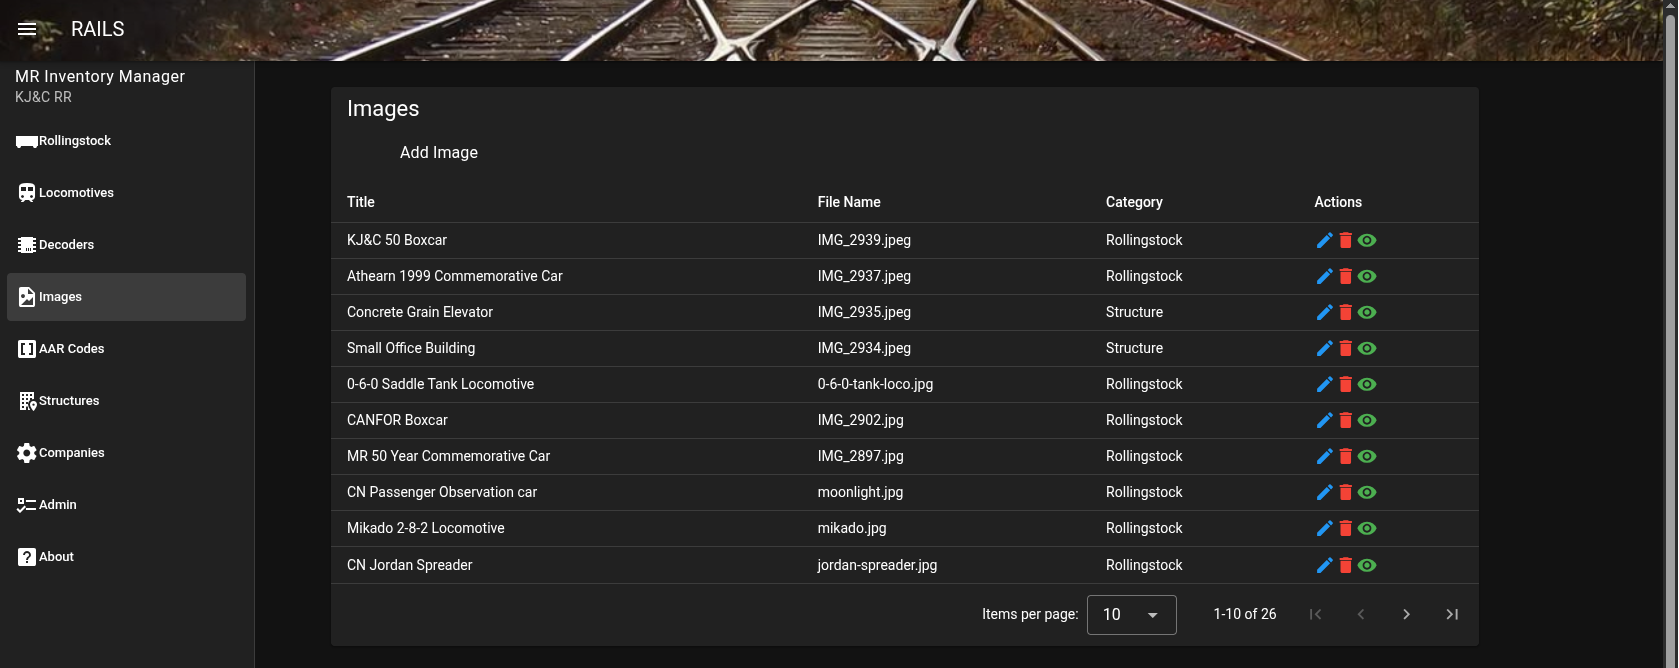
\includegraphics[width=0.85\textwidth]{./images/images.png}
    \caption{Images Page}
    \label{fig:images}
\end{figure}

\subsection{Viewing Image Details}

Clicking the green eye icon under the Actions column opens a modal dialog showing full metadata and a visual preview of the selected assetimages. The dialog presents the Title, File Name, Category, optional Notes, and an embedded image preview. Figure \ref{fig:images-view} shows the image viewer dialog.

\begin{figure}[H]
    \centering
    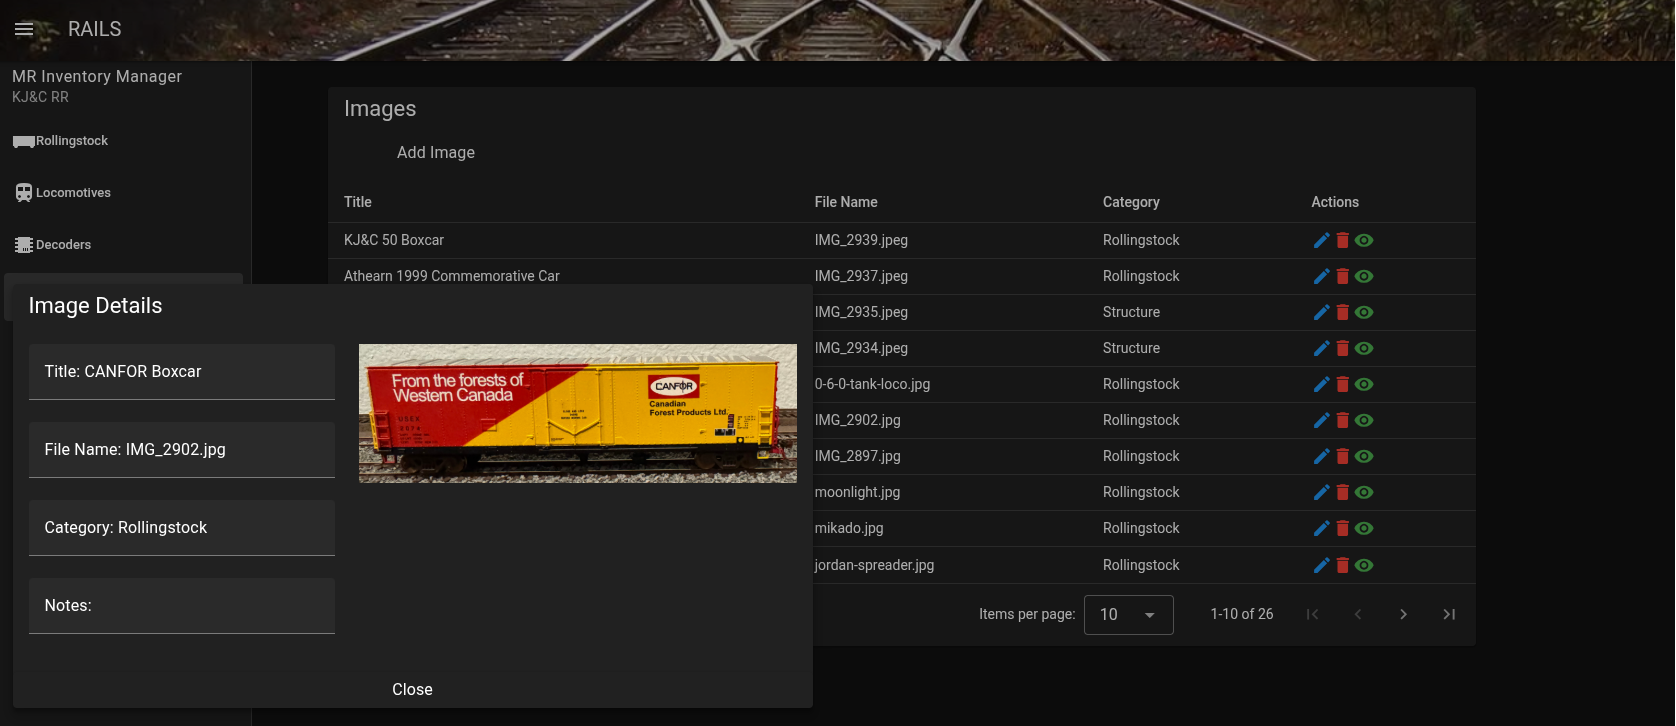
\includegraphics[width=0.85\textwidth]{./images/images-view.png}
    \caption{View Image Details}
    \label{fig:images-view}
\end{figure}

\subsection{Adding a New Image}

Clicking the "Add Image" button above the table opens a modal form for registering and uploading new graphic filesimages. The form prompts for a Title, a local File input path, a Category assignment, and optional Notes. Figure \ref{fig:images-new} illustrates the upload modal.

\begin{figure}[H]
    \centering
    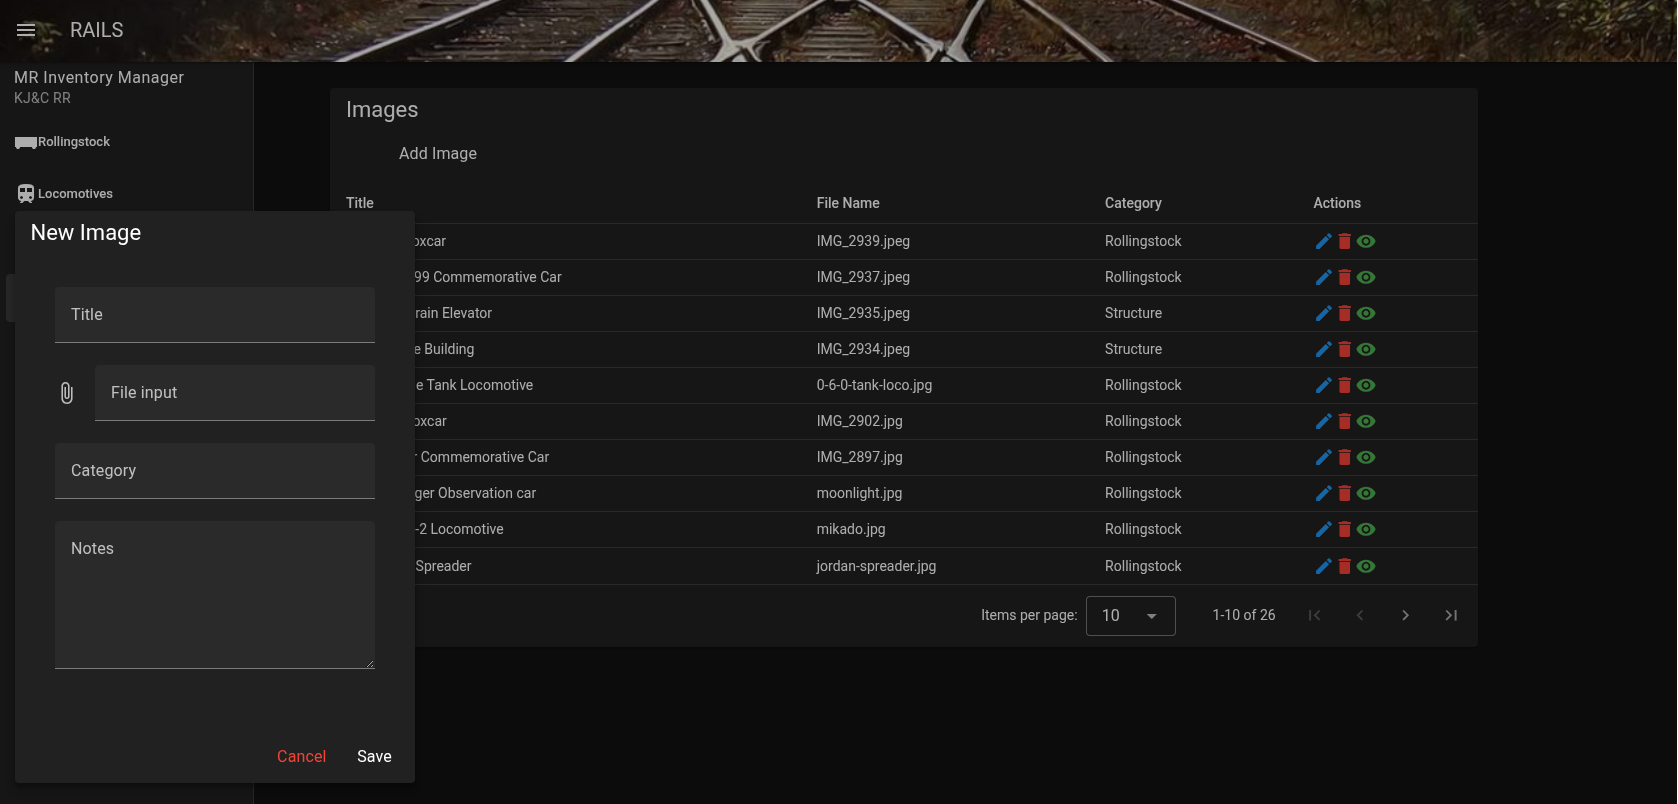
\includegraphics[width=0.85\textwidth]{./images/images-new.png}
    \caption{Add Image Dialog}
    \label{fig:images-new}
\end{figure}

\subsection{Editing Image Metadata}

To modify an existing image entry's descriptive metadata, click the blue pencil icon in the Actions columnimages. This opens the image dialog pre-populated with current values, allowing edits to the Title, File Name, Category, and Notes. Figure \ref{fig:images-edit} shows the edit dialog.

\begin{figure}[H]
    \centering
    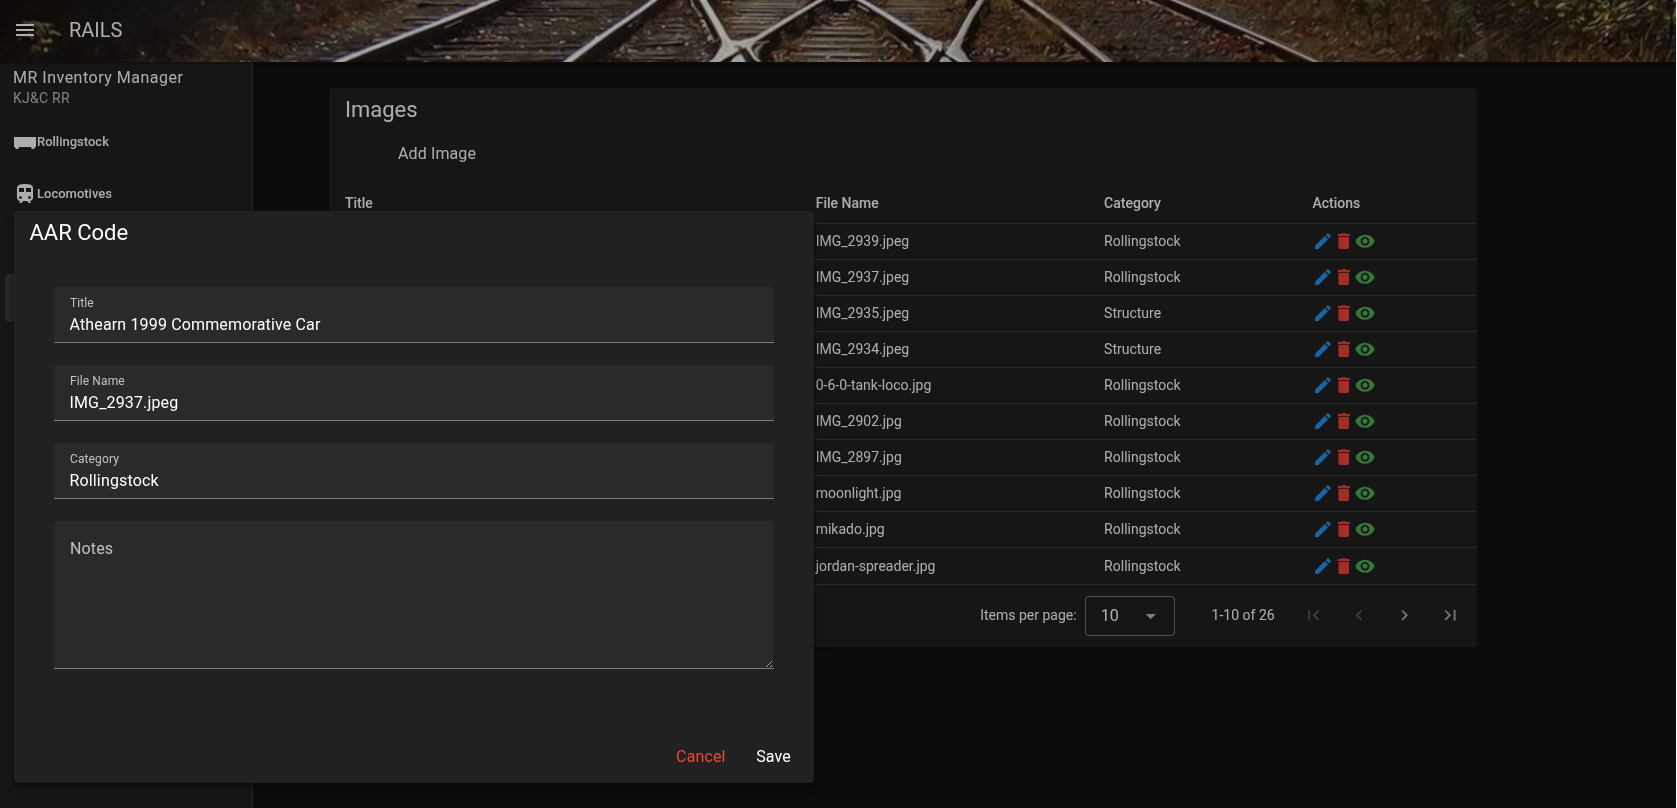
\includegraphics[width=0.85\textwidth]{./images/images-edit.png}
    \caption{Edit Image Metadata}
    \label{fig:images-edit}
\end{figure}

\subsection{Deleting Image Records}

To remove an image from the database repository, click the red trash bin icon under the Actions columnimages. A modal confirmation prompt appears requesting verification before the image asset record is deleted. Figure \ref{fig:images-delete} displays the deletion confirmation prompt.

\begin{figure}[H]
    \centering
    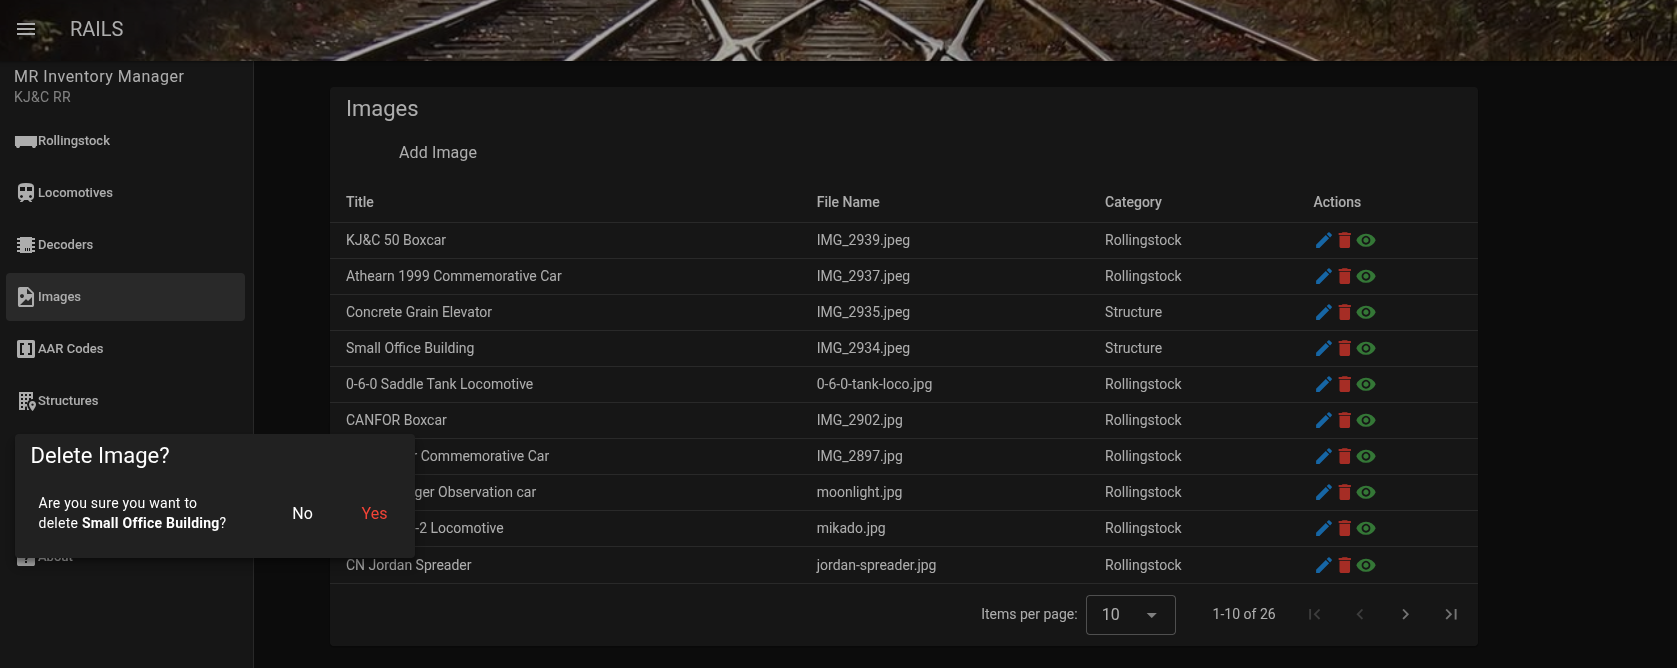
\includegraphics[width=0.85\textwidth]{./images/images-delete.png}
    \caption{Delete Image Confirmation}
    \label{fig:images-delete}
\end{figure}
